\begin{enumerate}
	\item L'administrateur se connecte au site avec ses identifiant. 
	\item Un nouveau bouton de navigation apparait dans la bar de navigation. 
	\item L'administrateur clique sur le bouton \textit{Admin}
	\item Il sélectionne \textit{Type Session} dans le menu déroulant. 
	\item L'administrateur atterris sur la page de gestion des type de sessions. 
	\item Il clique sur le bouton supprimer
	\item Une fenêtre de confirmation apparait. 
	\item Il clique sur \textit{OUI!} 
\end{enumerate}


\begin{figure}[h]
	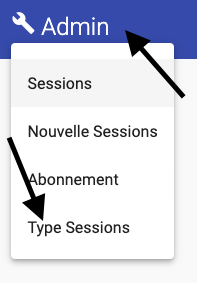
\includegraphics[width=0.4\textwidth,center]{Figures/us13-1}
	\caption{Menu de l'administrateur}
\end{figure}

\vspace{\baselineskip}
\begin{figure}[h]
	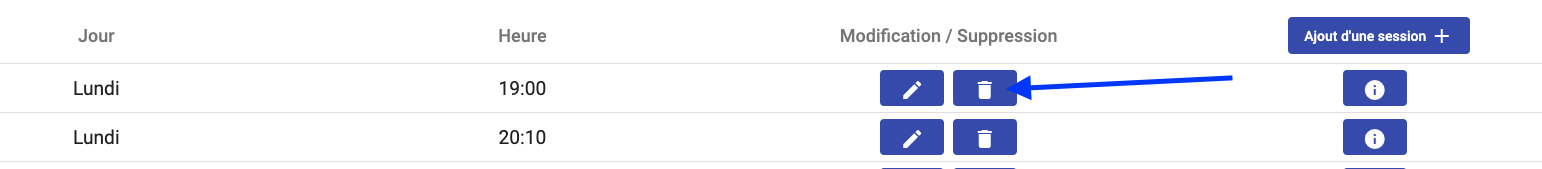
\includegraphics[width=0.9\textwidth,center]{Figures/us14-1}
	\caption{Bouton de suppression du type de session}
\end{figure}

\newpage
\begin{figure}[h]
	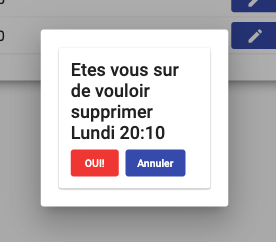
\includegraphics[width=0.4\textwidth,center]{Figures/us14-2}
	\caption{Fenêtre de confirmation de suppression}
\end{figure}

\subsubsection{Script concerné}
	\begin{itemize}
		\item \href{https://github.com/victorsmits/Aquabike/blob/master/backend/src/Controller/API/RegistrationControllerApi.php}{RegistrationControllerApi.php}
		\item \href{https://github.com/victorsmits/Aquabike/blob/master/backend/src/Entity/TypeSession.php}{TypeSession.php}
		\item \href{https://github.com/victorsmits/Aquabike/blob/master/frontend/src/app/type-session/del-type-session.component.ts}{del-type-session.component.ts}
		\item \href{https://github.com/victorsmits/Aquabike/blob/master/frontend/src/app/type-session/del-type-session.component.html}{del-type-session.component.html}
	\end{itemize}
